\section{Placement}

The placement of the I/O routers in a large 3D torus can have an enormous impact
on the traffic patterns and congestions characteristics present in the system.
This is important for maximizing I/O performance as well as minimizing the
interaction between application communication and I/O. Building on the lessons
learned from OLCF's Spider I implementation of fine-grained routing in 2008, an
improved method for placing LNET routers on Titan was developed and implemented
for Spider II.

\subsection{Topological Concerns}

The router placement layout used for Spider I was designed to distribute the
routers topologically through the machine while also minimizing the number of
cabinets that contained routers. This resulted in a very regular I/O pattern
that was prone to congestion if I/O traffic was not properly kept localized.

Jaguar's upgrade from Cray's SeaStar interconnect to Gemini changed the
network's characteristics.  Each Gemini supports two nodes, which effectively
halved the Y-dimension length.  Additionally, Y-dimension connections are
comprised of only half the links of X- and Z-dimension connections.  Thus, I/O
traffic should be limited in the Y-dimension due to its reduced relative
bandwidth. This suggests that routing zones should be ``flattened'' into
``rectangular prisms'' instead of the more traditional cubic zones.

Paper in \cite{interconnect}

Minimizing the hop count between clients and routers is essential for providing
high-bandwidth communications with the storage servers.  While Gemini routing
arbitration is locally fair, it is globally unfair.  Packet age and hop-count
are not taken into account when the router selects the next packet to forward.
Figure \ref{fig:geombw} shows an example of this issue.

Node 0 can be considered an I/O router while the others are acting as clients
attempting to send data to te router.  When only node 0 is communicating, it is
able to achieve 100\% of the bandwidth across the link.  Once node 2 starts
communicating, the router attached to node 1 accepts half the bandwidth from
node 1 and half from node 2.  Effectively, the bandwidth is shared between the
nodes.  When node 3 begins communicating, the router attached to node 2 fairly
arbitrates traffic between nodes 2 and 3.  Since that router only has half of
the global bandwith, nodes 2 and 3 each only get one quarter of the total
bandwith.  When node 4 begins communicating, the problem becomes even more
obvious.  The router attached to node 3 fairly arbitrates traffic between nodes
3 and 4, but it can only grant one eighth of the total bandwidth to each.


\begin{figure}[h]
  \centering
  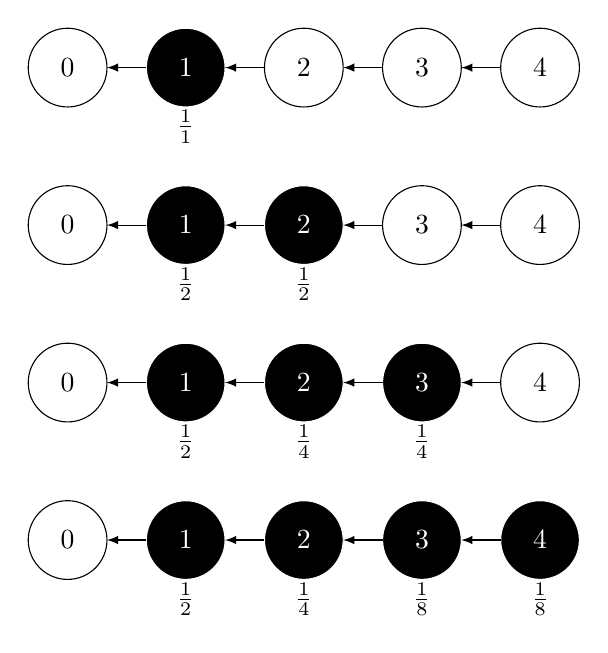
\begin{tikzpicture}
    \def \phase {1}
    \node[draw, circle, minimum height=1cm] at (0,-\phase){$0$};
    \node[draw, circle, minimum height=1cm, color=white, fill=black] at (1.5,-\phase){$1$};
    \node[draw, circle, minimum height=1cm] at (3,-\phase){$2$};
    \node[draw, circle, minimum height=1cm] at (4.5,-\phase){$3$};
    \node[draw, circle, minimum height=1cm] at (6,-\phase){$4$};
    \draw[->, >=latex] (1.0,-\phase) to (0.5,-\phase);
    \draw[->, >=latex] (2.5,-\phase) to (2.0,-\phase);
    \draw[->, >=latex] (4.0,-\phase) to (3.5,-\phase);
    \draw[->, >=latex] (5.5,-\phase) to (5.0,-\phase);
    \node[draw=none] at (1.5,-1.75) {$\frac{1}{1}$};

    \def \phase {3}
    \node[draw, circle, minimum height=1cm] at (0,-\phase){$0$};
    \node[draw, circle, minimum height=1cm, color=white, fill=black] at (1.5,-\phase){$1$};
    \node[draw, circle, minimum height=1cm, color=white, fill=black] at (3,-\phase){$2$};
    \node[draw, circle, minimum height=1cm] at (4.5,-\phase){$3$};
    \node[draw, circle, minimum height=1cm] at (6,-\phase){$4$};
    \draw[->, >=latex] (1.0,-\phase) to (0.5,-\phase);
    \draw[->, >=latex] (2.5,-\phase) to (2.0,-\phase);
    \draw[->, >=latex] (4.0,-\phase) to (3.5,-\phase);
    \draw[->, >=latex] (5.5,-\phase) to (5.0,-\phase);
    \node[draw=none] at (1.5,-3.75) {$\frac{1}{2}$};
    \node[draw=none] at (3,-3.75) {$\frac{1}{2}$};

    \def \phase {5}
    \node[draw, circle, minimum height=1cm] at (0,-\phase){$0$};
    \node[draw, circle, minimum height=1cm, color=white, fill=black] at (1.5,-\phase){$1$};
    \node[draw, circle, minimum height=1cm, color=white, fill=black] at (3,-\phase){$2$};
    \node[draw, circle, minimum height=1cm, color=white, fill=black] at (4.5,-\phase){$3$};
    \node[draw, circle, minimum height=1cm] at (6,-\phase){$4$};
    \draw[->, >=latex] (1.0,-\phase) to (0.5,-\phase);
    \draw[->, >=latex] (2.5,-\phase) to (2.0,-\phase);
    \draw[->, >=latex] (4.0,-\phase) to (3.5,-\phase);
    \draw[->, >=latex] (5.5,-\phase) to (5.0,-\phase);
    \node[draw=none] at (1.5,-5.75) {$\frac{1}{2}$};
    \node[draw=none] at (3,-5.75) {$\frac{1}{4}$};
    \node[draw=none] at (4.5,-5.75) {$\frac{1}{4}$};

    \def \phase {7}
    \node[draw, circle, minimum height=1cm] at (0,-\phase){$0$};
    \node[draw, circle, minimum height=1cm, color=white, fill=black] at (1.5,-\phase){$1$};
    \node[draw, circle, minimum height=1cm, color=white, fill=black] at (3,-\phase){$2$};
    \node[draw, circle, minimum height=1cm, color=white, fill=black] at (4.5,-\phase){$3$};
    \node[draw, circle, minimum height=1cm, color=white, fill=black] at (6,-\phase){$4$};
    \draw[->, >=latex] (1.0,-\phase) to (0.5,-\phase);
    \draw[->, >=latex] (2.5,-\phase) to (2.0,-\phase);
    \draw[->, >=latex] (4.0,-\phase) to (3.5,-\phase);
    \draw[->, >=latex] (5.5,-\phase) to (5.0,-\phase);
    \node[draw=none] at (1.5,-7.75) {$\frac{1}{2}$};
    \node[draw=none] at (3,-7.75) {$\frac{1}{4}$};
    \node[draw=none] at (4.5,-7.75) {$\frac{1}{8}$};
    \node[draw=none] at (6,-7.75) {$\frac{1}{8}$};
  \end{tikzpicture}
  \caption{Geometric Bandwidth Reductions}\label{fig:geombw}
\end{figure}

As these chains get longer and longer, the bandwidth available to the ``last''
node can become abysmal.

Minimize torus congestion

GPUs has increased load on network

Congestion avoidance

\subsection{Physical Constraints}

As part of the Spider II upgrade, the number of LNET routers on Titan was
doubled to 440 nodes and each router was equipped with an IB FDR HCA with 16
PCI-E lanes running at Gen-2.

Ensure full routability to boot from both ends

Balance router usage

Minimize Pinging

Swizzle to spread Gemini load

\subsection{Implementation}


% vim:textwidth=80:
